% Informe tecnico del Proyecto Final 2026
% Catedra de IA aplicada a Robotica Movil - FIUNA
%
% Escrito sobre la plantilla de la catedra (formato Springer Nature, clase
% sn-jnl.cls). Compilar dos veces:  pdflatex informe_tecnico.tex
% Las figuras de datos se regeneran con:  python generar_figuras.py

\documentclass[pdflatex,sn-mathphys-num]{sn-jnl}

% -----------------------------------------------------------------------------
% Paquetes
% -----------------------------------------------------------------------------
\usepackage[utf8]{inputenc}
\usepackage[T1]{fontenc}
% babel solo para la separacion en silabas del castellano: con es-nolayout,
% es-nosectiondot y es-noindentfirst no altera el formato de la plantilla.
\usepackage[spanish,es-tabla,es-noquoting,es-noshorthands,es-nodecimaldot,es-nolayout,es-nosectiondot,es-noindentfirst]{babel}
\usepackage{graphicx}
\usepackage{amsmath,amssymb,amsfonts}
\usepackage{xcolor}
\usepackage{booktabs}
\usepackage{array}
\usepackage{listings}
\usepackage{fancyhdr}
\usepackage{url}
\usepackage[title]{appendix}
\usepackage{tikz}
\usetikzlibrary{positioning,arrows.meta,fit,backgrounds}

\renewcommand{\abstractname}{Resumen}
\renewcommand{\figurename}{Figura}
\renewcommand{\tablename}{Tabla}
\renewcommand{\refname}{Referencias}
\renewcommand{\appendixname}{Ap\'endice}
\providecommand{\keywordname}{Keywords}
\renewcommand{\keywordname}{Palabras clave}

\graphicspath{{figuras/}}
\newcolumntype{L}[1]{>{\raggedright\arraybackslash}p{#1}}
\newcommand{\cod}[1]{\texttt{#1}}
\newcommand{\grad}{\ensuremath{^\circ}}

% -----------------------------------------------------------------------------
% Datos institucionales y encabezado
% -----------------------------------------------------------------------------
\newcommand{\institucion}{Facultad de Ingenier\'ia -- Universidad Nacional de Asunci\'on}
\newcommand{\catedra}{C\'atedra de Inteligencia Artificial aplicada a la Rob\'otica}
\newcommand{\proyecto}{Proyecto Final -- 2026}

\setlength{\headheight}{42pt}
\setlength{\headsep}{18pt}
\pagestyle{fancy}
\fancyhf{}
\fancyhead[C]{%
  \footnotesize
  \textbf{\institucion}\\[-1pt]
  \catedra\\[-1pt]
  \proyecto
}
\fancyfoot[C]{\thepage}
\renewcommand{\headrulewidth}{0.4pt}
\renewcommand{\footrulewidth}{0pt}

% La primera pagina generada por \maketitle utiliza el estilo plain.
\fancypagestyle{plain}{%
  \fancyhf{}
  \fancyhead[C]{%
    \footnotesize
    \textbf{\institucion}\\[-1pt]
    \catedra\\[-1pt]
    \proyecto
  }
  \fancyfoot[C]{\thepage}
  \renewcommand{\headrulewidth}{0.4pt}
  \renewcommand{\footrulewidth}{0pt}
}

% -----------------------------------------------------------------------------
% Configuracion de enlaces y codigo
% -----------------------------------------------------------------------------
\definecolor{azulFIUNA}{RGB}{0,74,128}
\definecolor{grisCodigo}{RGB}{247,247,247}
\definecolor{azul}{HTML}{2A78D6}
\definecolor{naranja}{HTML}{EB6834}
\definecolor{gris}{HTML}{52514E}
\definecolor{verde}{HTML}{0CA30C}
\hypersetup{
  colorlinks=true,
  linkcolor=azulFIUNA,
  citecolor=azulFIUNA,
  urlcolor=azulFIUNA
}

\lstset{
  basicstyle=\ttfamily\small,
  backgroundcolor=\color{grisCodigo},
  frame=single,
  rulecolor=\color{black!25},
  numbers=left,
  numberstyle=\scriptsize\color{black!60},
  breaklines=true,
  showstringspaces=false,
  tabsize=4,
  captionpos=b
}
\renewcommand{\lstlistingname}{Listado}

\raggedbottom

% La clase une a los dos ultimos autores con "and"; aqui se lo pasa a "y".
\makeatletter
\def\au@and{\ifnum\punctcount=2\ y\else\unskip, \advance\punctcount by -1 \fi}
\makeatother

% =============================================================================
\begin{document}

\title[Aguar\'a: aproximaci\'on y evasi\'on con visi\'on a bordo]{Aguar\'a: robot
m\'ovil aut\'onomo de aproximaci\'on y evasi\'on basado en detecci\'on de objetos
con una red neuronal ejecutada a bordo}
\subtitle{\small{Proyecto Final -- C\'atedra de Inteligencia Artificial aplicada a la Rob\'otica}}

\author[1]{\fnm{Federico} \sur{Mor\'an}}
\email{federico.moran@uc.edu.py}

% Falta el correo del segundo autor: agregar aqui  \email{...}
\author[1]{\fnm{Juan} \sur{Barboza}}
\email{juan.barboza@uc.edu.py}

\affil[1]{%
  \orgdiv{Maestr\'ia en Ciencias de la Inteligencia Artificial},
  \orgname{Facultad de Ingenier\'ia, Universidad Nacional de Asunci\'on},
  \orgaddress{\city{San Lorenzo}, \country{Paraguay}}
}

\abstract{%
Se presenta el dise\~no, la construcci\'on y la evaluaci\'on de Aguar\'a, un robot
m\'ovil de tracci\'on diferencial que busca un objeto objetivo, se aproxima a \'el y evade
otro, considerado amenaza, decidiendo todo a bordo. La
percepci\'on usa la red de detecci\'on YOLOv8n, preentrenada en COCO y
ejecutada en la CPU de una Raspberry Pi 5; una m\'aquina
de cuatro estados arbitra el comportamiento, con prioridad incondicional de la
evasi\'on, y una ley de control proporcional sobre la imagen genera las
consignas de avance y giro. Un microcontrolador ESP32 las traduce a potencia
para cada rueda, mide la distancia frontal con un sensor ultras\'onico y
detiene los motores si deja de recibir \'ordenes. El sistema se evalu\'o con
79 verificaciones autom\'aticas sin hardware y con 24 corridas registradas en
el piso. El lazo completo opera a unas 10 im\'agenes por segundo, con unos
150 ms de latencia. El
robot confirma un objeto 0,2 s despu\'es de verlo, alcanza el objetivo desde
1 m en 2 a 3 s y se detiene a unos 30 cm; ante la amenaza inicia la maniobra de
evasi\'on en 0,2 s y, con el sensor ultras\'onico, interrumpe el avance ante obstáculos. Se discuten sus limitaciones.
}

\keywords{rob\'otica m\'ovil, detecci\'on de objetos, YOLOv8, sistemas embebidos, rob\'otica basada en comportamientos, control visual}

\maketitle

% -----------------------------------------------------------------------------
\section{Introducci\'on}\label{sec:introduccion}

La detecci\'on de objetos con redes convolucionales de una sola etapa permite
hoy que un robot peque\~no reconozca lo que tiene delante con una c\'amara
com\'un~\cite{ref:yolo,ref:yolorev}. El paso que sigue, y que interesa a la
rob\'otica m\'ovil, es cerrar el lazo: que esa detecci\'on se convierta en una
decisi\'on y en un movimiento, en tiempo real y sin una computadora externa.
Ese paso obliga a resolver problemas que no aparecen al evaluar la red sobre
un conjunto de im\'agenes: el retardo entre la imagen y la acci\'on, la
p\'erdida moment\'anea de las detecciones, los actuadores que no responden de
forma ideal y la alimentaci\'on de un c\'omputo exigente con bater\'ias.

Este trabajo aborda ese problema con un robot diferencial de bajo costo que
exhibe dos conductas opuestas ante dos objetos: se aproxima a uno y huye del
otro. Se lo denomin\'o \emph{Aguar\'a}, ``zorro'' en guaran\'i, por el animal
que se acerca a lo que busca y escapa de lo que lo amenaza. El caso es deliberadamente simple en lo perceptivo ---dos clases de un
modelo preentrenado--- para concentrar el esfuerzo en la integraci\'on de la
percepci\'on con el control y en su medici\'on sobre el robot f\'isico.

Las contribuciones principales son: (i) una arquitectura de dos niveles, con
una frontera expl\'icita entre el c\'omputo que decide y el que act\'ua, y un
freno autom\'atico independiente de la capa de decisi\'on; (ii) una m\'aquina
de estados con arbitraje de conflictos, verificable por completo sin hardware;
(iii) una calibraci\'on de la tracci\'on por rueda que compensa dos motores
con caracter\'isticas distintas sin usar codificadores; y (iv) un registro
ciclo por ciclo de cada corrida, que permite reconstruir cada decisi\'on y que
sostiene los resultados que aqu\'i se informan.

El resto del informe se organiza as\'i: la Secci\'on~\ref{sec:diseno} describe
el dise\~no y la implementaci\'on; la Secci\'on~\ref{sec:metodologia}, la
metodolog\'ia de evaluaci\'on; la Secci\'on~\ref{sec:resultados} presenta y
discute los resultados, y la Secci\'on~\ref{sec:conclusiones} resume las
conclusiones y el trabajo futuro.

\subsection{Planteamiento del problema y objetivos}\label{subsec:problema}

El escenario es un ambiente interior de piso liso y despejado, de unos pocos
metros de lado. En \'el se colocan dos objetos: un \emph{objetivo}, que es un
oso de peluche impreso en una hoja A4 (unos 20 cm de ancho), y una
\emph{amenaza}, que es una mochila real. El robot arranca en una posici\'on y
orientaci\'on cualesquiera y no conoce la ubicaci\'on de los objetos.

Las restricciones son las siguientes. Todo el c\'omputo se realiza a bordo, sin
red ni teleoperaci\'on; la inferencia corre en la CPU de una Raspberry Pi 5, sin
acelerador; los motores son de corriente continua con reductora, sin lazo de
velocidad; la c\'amara es una c\'amara web USB fija, a unos 10 cm del piso, y el
robot se alimenta con bater\'ias.

\subsubsection{Objetivo general}

Dise\~nar, construir y evaluar un robot m\'ovil aut\'onomo que, mediante
detecci\'on de objetos con una red neuronal ejecutada a bordo, busque un objeto
objetivo, se aproxime a \'el y se detenga a una distancia definida, y que evada
un objeto amenaza, dando prioridad a la evasi\'on cuando ambos est\'an a la
vista.

\subsubsection{Objetivos espec\'ificos}

\begin{itemize}
  \item Ejecutar la detecci\'on de objetos en la Raspberry Pi 5 a no menos de
        5 im\'agenes por segundo dentro del lazo completo de percepci\'on,
        decisi\'on y actuaci\'on.
  \item Implementar una m\'aquina de estados con las conductas de b\'usqueda,
        aproximaci\'on, llegada y evasi\'on, y con un arbitraje expl\'icito que
        d\'e prioridad a la evasi\'on.
  \item Dise\~nar una ley de control que centre el objetivo en la imagen y
        detenga el robot a una distancia definida, usando s\'olo la caja
        delimitadora que entrega la red.
  \item Desarrollar el control de bajo nivel en un microcontrolador, con
        compensaci\'on de las diferencias entre motores y un mecanismo de
        parada segura ante la p\'erdida de comunicaci\'on.
  \item Incorporar un sensor de distancia para evitar el avance contra
        obst\'aculos y una se\~nal sonora de los eventos.
  \item Medir el desempe\~no del sistema en el robot f\'isico: velocidad de
        procesamiento, latencias, alcance de detecci\'on, tiempos y \'exito de
        cada conducta.
\end{itemize}

\subsection{Fundamentos y trabajos relacionados}\label{subsec:fundamentos}

\textbf{Detecci\'on de objetos.} Los detectores de una etapa de la familia
YOLO plantean la detecci\'on como una \'unica regresi\'on desde la imagen
hacia cajas delimitadoras y probabilidades de clase, lo que los hace aptos
para tiempo real~\cite{ref:yolo}. YOLOv8~\cite{ref:yolov8} es una versi\'on sin
anclas de esa familia, con variantes de distinto tama\~no; la m\'as chica
(\emph{nano}, YOLOv8n) tiene unos 3 millones de par\'ametros~\cite{ref:yolorev}.
Los pesos que se distribuyen est\'an entrenados en COCO~\cite{ref:coco}, un
conjunto con 80 clases de objetos cotidianos fotografiados en su contexto
habitual. Esta \'ultima caracter\'istica result\'o relevante: las mochilas de
COCO aparecen en su mayor\'ia sobre la espalda de una persona y vistas a su
altura, no apoyadas en el piso y vistas desde abajo
(Secci\'on~\ref{subsec:discusion}).

\textbf{Rob\'otica basada en comportamientos.} La idea de que conductas
simples y reactivas, conectadas casi directamente de los sensores a los
motores, producen un comportamiento aparentemente dirigido aparece en los
veh\'iculos de Braitenberg~\cite{ref:braitenberg}, cuyos casos can\'onicos son
justamente la atracci\'on y la huida. La arquitectura de
subsunci\'on~\cite{ref:brooks} organiza esas conductas en capas, donde las de
mayor prioridad inhiben a las dem\'as; el arbitraje por prioridad fija entre
conductas es el esquema m\'as simple de coordinaci\'on en este
paradigma~\cite{ref:arkin}. En este trabajo la evasi\'on subsume a la
aproximaci\'on.

\textbf{Control visual.} El control basado en imagen regula directamente
caracter\'isticas medidas en el plano de la imagen, sin reconstruir la
posici\'on del objeto en el espacio~\cite{ref:visualservo}. Aqu\'i se usan dos
caracter\'isticas de la caja delimitadora: su posici\'on horizontal, para el
giro, y su \'area, para el avance.

\textbf{Locomoci\'on diferencial.} El modelo cinem\'atico de un robot de dos
ruedas motrices independientes relaciona las velocidades de las ruedas con
la velocidad lineal y la angular del veh\'iculo~\cite{ref:siegwart}; es el
modelo que usa el microcontrolador para mezclar las consignas.

Respecto de las soluciones habituales, que ejecutan la inferencia en una GPU
embebida o en una computadora externa, o que reentrenan la red para sus
propios objetos, esta propuesta se limita a un modelo preentrenado y a la CPU
de la Raspberry Pi. El aporte no est\'a en la red, sino en su integraci\'on en
un lazo de control f\'isico y en la medici\'on de ese lazo.

\section{Dise\~no e implementaci\'on del sistema}\label{sec:diseno}

\subsection{Arquitectura general}

El sistema tiene dos niveles (Figura~\ref{fig:arquitectura}). El nivel alto
corre en la Raspberry Pi 5: captura una imagen, ejecuta la red, actualiza la
m\'aquina de estados y calcula una consigna de movimiento. El nivel bajo corre
en un ESP32: recibe la consigna por un enlace serie, la convierte en una
se\~nal de potencia para cada rueda, lee el sensor ultras\'onico, maneja el
zumbador y devuelve telemetr\'ia.

\begin{figure}[htbp]
  \centering
  \begin{tikzpicture}[font=\footnotesize, >={Stealth[length=2mm]},
      b/.style={draw, rounded corners=2pt, minimum height=0.85cm, align=center,
                line width=0.7pt, text width=1.75cm, inner sep=2pt}]
    \node[b, draw=azul, fill=azul!8] (cam) {C\'amara\\USB};
    \node[b, draw=azul, fill=azul!8, right=0.35cm of cam] (yolo) {Red\\YOLOv8n};
    \node[b, draw=azul, fill=azul!8, right=0.35cm of yolo] (conf) {Confirmaci\'on\\temporal};
    \node[b, draw=azul, fill=azul!8, right=0.35cm of conf] (est) {M\'aquina de\\estados};
    \node[b, draw=azul, fill=azul!8, right=0.35cm of est] (ctl) {Ley de\\control};
    \begin{scope}[on background layer]
      \node[draw=azul, dashed, rounded corners=4pt, fit=(cam)(ctl), inner sep=7pt,
            label={[azul]above:\textbf{Raspberry Pi 5: decide, $\sim$10 ciclos por segundo}}] (pi) {};
    \end{scope}
    \node[b, draw=naranja, fill=naranja!8, below=1.9cm of ctl] (mez) {Mezcla y\\calibraci\'on};
    \node[b, draw=naranja, fill=naranja!8, left=0.35cm of mez] (wd) {Freno\\autom\'atico};
    \node[b, draw=gris, fill=gris!8, left=0.35cm of wd] (mot) {L298N y\\motores};
    \node[b, draw=naranja, fill=naranja!8, left=0.35cm of mot] (son) {Ultras\'onico};
    \node[b, draw=naranja, fill=naranja!8, left=0.35cm of son] (buz) {Zumbador};
    \begin{scope}[on background layer]
      \node[draw=naranja, dashed, rounded corners=4pt, fit=(buz)(mez), inner sep=7pt,
            label={[naranja]below:\textbf{ESP32: ejecuta, 100 ciclos por segundo}}] (esp) {};
    \end{scope}
    \draw[->] (cam) -- (yolo); \draw[->] (yolo) -- (conf);
    \draw[->] (conf) -- (est); \draw[->] (est) -- (ctl);
    \draw[->, line width=1pt] ([xshift=6pt]ctl.south) --
        node[right, align=left]{\cod{M,v\_lin,v\_ang}\\\cod{B,patr\'on}} ([xshift=6pt]mez.north);
    \draw[->, line width=1pt] ([xshift=-6pt]son.north) |- ++(0,0.75) -|
        node[pos=0.25, above]{\cod{D,distancia,\ldots} (20 por segundo)} (est.south);
    \draw[->] (mez) -- (wd); \draw[->] (wd) -- (mot);
  \end{tikzpicture}
  \caption{Arquitectura general. La Raspberry Pi nunca maneja un motor y el
  ESP32 nunca toma una decisi\'on de comportamiento. Entre ambos viaja una
  consigna de intenci\'on (avance y giro, de $-100$ a $100$) y vuelve la
  distancia medida.}
  \label{fig:arquitectura}
\end{figure}

Las decisiones de dise\~no que definen esta arquitectura son las siguientes.

\begin{itemize}
  \item \textbf{Un solo microcontrolador de bajo nivel.} Se descart\'o
        combinar dos microcontroladores: duplicaba el firmware y los
        protocolos sin aportar funcionalidad.
  \item \textbf{Modelo preentrenado, sin entrenamiento propio.} El ciclo de
        captura, etiquetado y entrenamiento a\~nad\'ia riesgo de cronograma sin
        ser el aporte buscado.
  \item \textbf{La compensaci\'on de los motores vive en el ESP32.} El nivel
        alto env\'ia una intenci\'on normalizada; s\'olo el microcontrolador
        conoce los valores de modulaci\'on de cada rueda. As\'i la ley de
        control no depende del hardware de tracci\'on.
  \item \textbf{Las capas que deciden no acceden al hardware.} La m\'aquina de
        estados y la ley de control reciben percepciones y un instante de
        tiempo como argumentos y devuelven una consigna; por eso pueden
        ejecutarse a velocidad de simulaci\'on y verificarse sin c\'amara ni
        robot.
  \item \textbf{Confirmaci\'on temporal.} Una detecci\'on aislada no cambia el
        estado: una clase se da por presente tras 3 im\'agenes consecutivas y
        por perdida tras 5 sin ella.
  \item \textbf{Parada segura en dos niveles.} Si el lazo de visi\'on se
        retrasa m\'as de 0,40 s, la Raspberry Pi env\'ia una consigna nula; si el
        ESP32 no recibe consignas durante 0,5 s, frena los motores por su
        cuenta.
\end{itemize}

\subsection{Componentes e implementaci\'on}

\subsubsection{Plataforma y electr\'onica}

La Tabla~\ref{tab:componentes} resume los componentes y la
Figura~\ref{fig:robot} muestra el robot terminado. La alimentaci\'on usa dos
fuentes independientes con masa com\'un: una bater\'ia port\'atil de 5 V para
la Raspberry Pi (y, por sus puertos USB, la c\'amara y el ESP32) y una fuente
de 12 V s\'olo para la etapa de potencia de los motores. La separaci\'on no fue
una decisi\'on inicial sino el resultado de una medici\'on
(Secci\'on~\ref{sec:resultados}).

\begin{table}[htbp]
  \caption{Componentes del robot.}
  \label{tab:componentes}
  \centering
  \begin{tabular}{@{}L{3.0cm}L{4.6cm}L{4.5cm}@{}}
    \toprule
    \textbf{Componente} & \textbf{Detalle} & \textbf{Funci\'on} \\
    \midrule
    Raspberry Pi 5 & 8 GB de RAM, sin monitor & Percepci\'on y decisi\'on \\
    ESP32 & Placa de desarrollo con puente USB-serie & Control de bajo nivel y seguridad \\
    Etapa de potencia & M\'odulo L298N, puente H doble~\cite{ref:l298} & Accionamiento de los motores \\
    Motores (2) & GM25-370, 12 V, con reductora & Tracci\'on diferencial \\
    Chasis & Dos ruedas de 60 mm y una rueda loca & Locomoci\'on \\
    C\'amara & C\'amara web USB, 640$\times$480, MJPEG & Detecci\'on de objetos \\
    Ultras\'onico & Parallax PING))), un pin de se\~nal~\cite{ref:ping} & Distancia frontal, 2 cm a 3 m \\
    Zumbador & Activo, de dos terminales & Se\~nalizaci\'on de eventos \\
    Bater\'ia port\'atil & 20\,000 mAh, 5 V / 3 A & Alimenta la Raspberry Pi \\
    Fuente de 12 V & 10\,000 mAh, con salida de 12 V & Alimenta s\'olo los motores \\
    \bottomrule
  \end{tabular}
\end{table}

\begin{figure}[htbp]
  \centering
  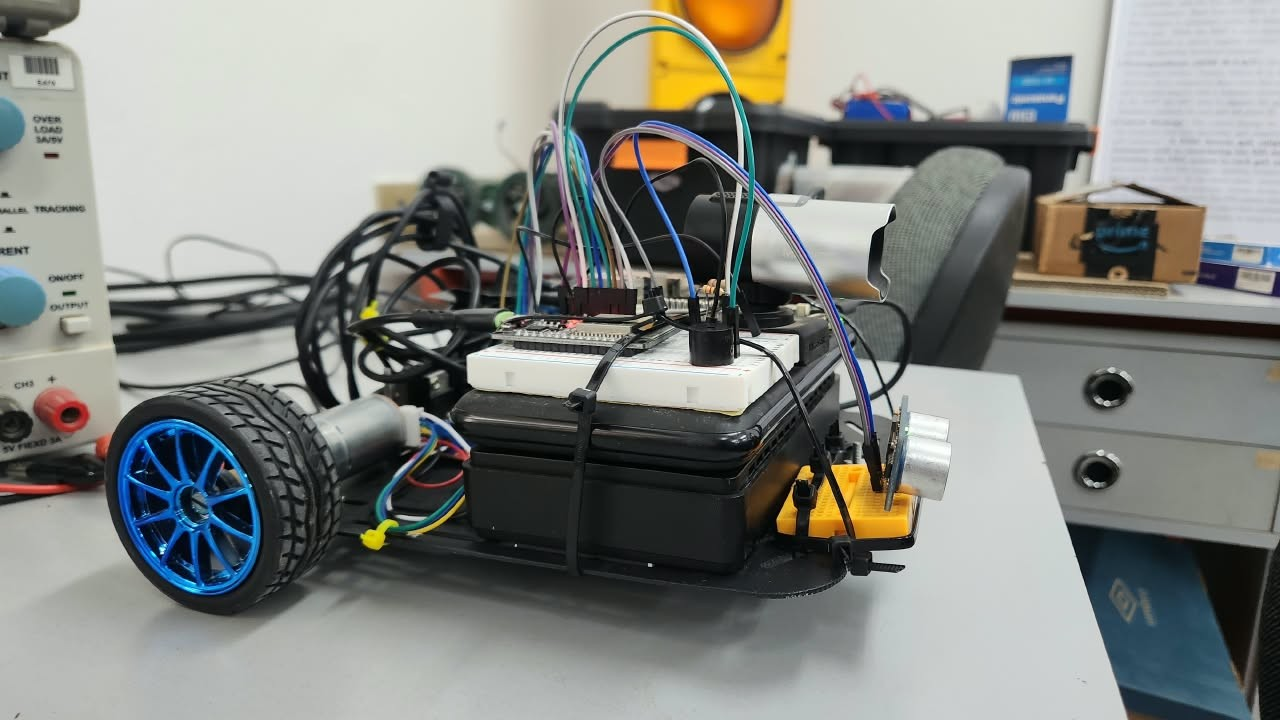
\includegraphics[height=3.75cm]{robot_terminado_lado.jpg}\hspace{2mm}%
  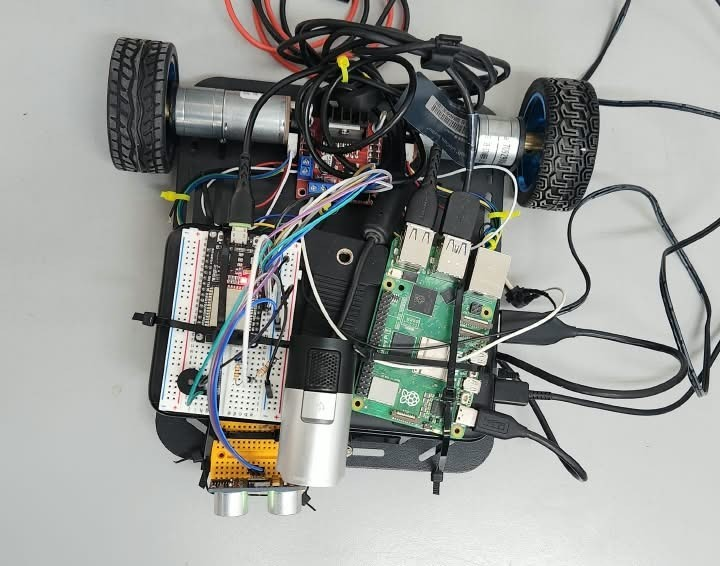
\includegraphics[height=3.75cm]{robot_terminado_arriba.jpg}
  \caption{El robot terminado. Al frente, el sensor ultras\'onico y, sobre
  \'el, la c\'amara; en la placa de pruebas, el ESP32 y el zumbador; a su lado,
  la Raspberry Pi 5; atr\'as, la etapa de potencia y los motores.}
  \label{fig:robot}
\end{figure}

El sensor ultras\'onico usa una sola l\'inea para el disparo y para el eco, y
la entrega a 5 V; como las entradas del ESP32 admiten 3,3 V~\cite{ref:esp32},
se intercala un divisor resistivo (1 k$\Omega$ en serie y 2 k$\Omega$ a masa).
El firmware configura el pin como salida para emitir el pulso de disparo y de
inmediato como entrada; una interrupci\'on mide el ancho del pulso de eco, de
modo que la medici\'on no bloquea el lazo de control.

\subsubsection{Control de bajo nivel y calibraci\'on de la tracci\'on}

El ESP32 recibe la consigna $(v_{lin}, v_{ang})$, con valores enteros entre
$-100$ y $100$, y la mezcla seg\'un el modelo diferencial~\cite{ref:siegwart}:
\begin{equation}
  u_{izq} = v_{lin} + v_{ang}, \qquad u_{der} = v_{lin} - v_{ang},
  \label{eq:mezcla}
\end{equation}
donde $v_{ang}>0$ significa girar a la derecha. Si alguna rueda supera el
rango, se escala el par completo para conservar la curvatura pedida.

Los dos motores, aunque del mismo modelo, resultaron distintos: una rueda
entrega 2,11 veces m\'as velocidad que la otra por unidad de ciclo de trabajo,
y sus umbrales de arranque tambi\'en difieren. Como no hay codificadores, la
compensaci\'on se hace a lazo abierto con una recta por rueda. Para un comando
normalizado $u\in(0,1]$, el ciclo de trabajo aplicado es
\begin{equation}
  d(u) = d_{\min} + u\,(d_{\max}-d_{\min}),
  \label{eq:duty}
\end{equation}
con un piso $d_{\min}$ y un techo $d_{\max}$ propios de cada rueda, medidos de
forma que ambas giren a la misma velocidad para el mismo $u$
(Figura~\ref{fig:calibracion}). Al pasar de reposo a movimiento se aplica un
pulso breve de mayor potencia para vencer la fricci\'on est\'atica. La
modulaci\'on es de 1 kHz y 10 bits.

\begin{figure}[htbp]
  \centering
  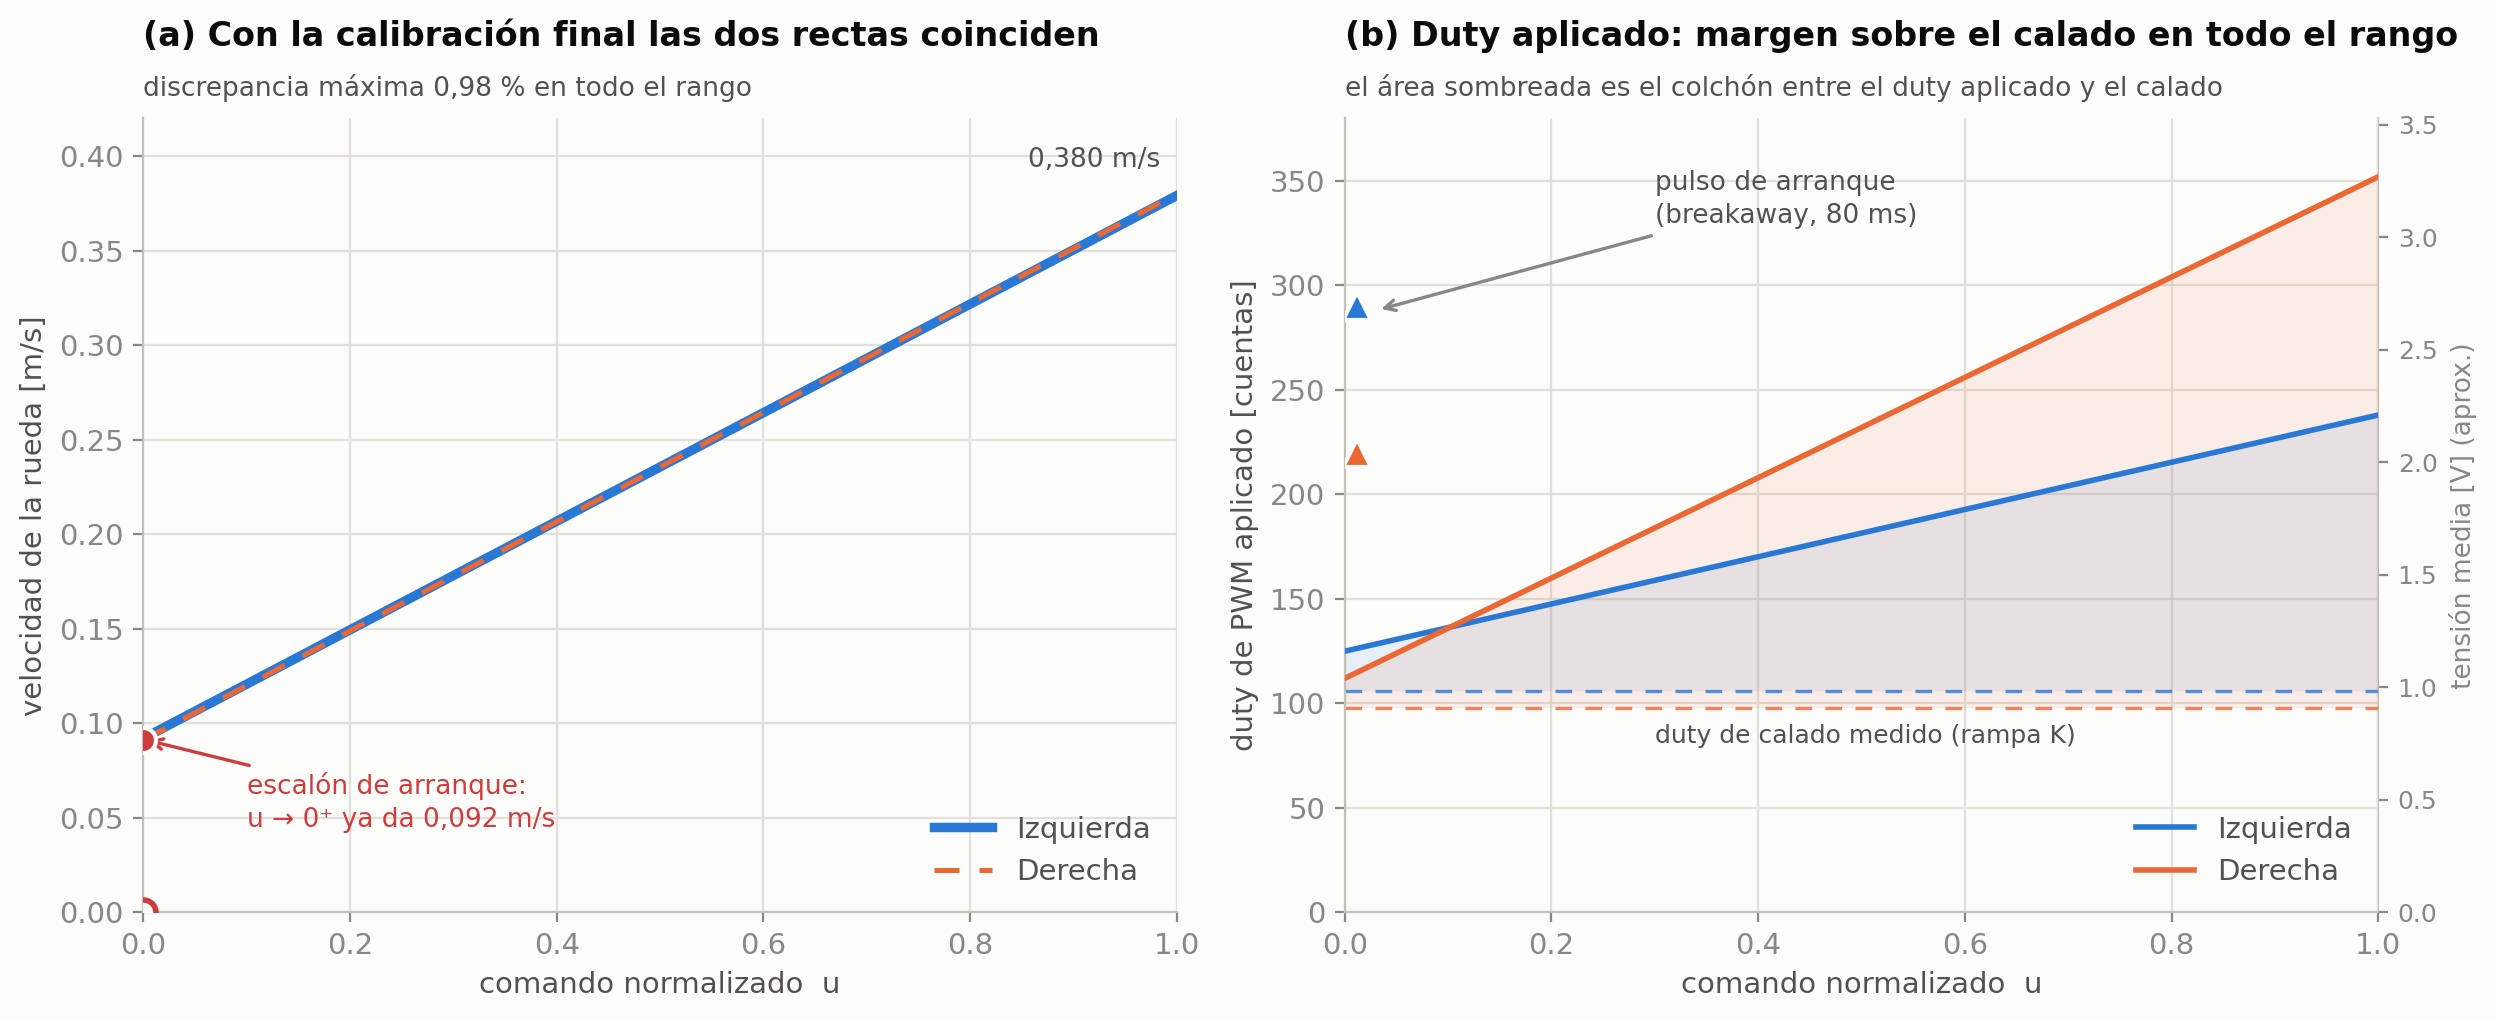
\includegraphics[width=0.98\textwidth]{calibracion_banco.png}
  \caption{Calibraci\'on de la tracci\'on con las ruedas en el aire. (a) Con
  una recta por rueda, las velocidades coinciden con una discrepancia m\'axima
  de 0,98~\%. (b) Ciclo de trabajo aplicado a cada rueda. Con el robot apoyado
  hubo que elevar pisos y techos (Tabla~\ref{tab:calibracion}).}
  \label{fig:calibracion}
\end{figure}

\subsubsection{Percepci\'on}

La red es YOLOv8n con los pesos de COCO, ejecutada con imagen de entrada de
320 p\'ixeles. Las clases de inter\'es se declaran por nombre: \cod{teddy
bear} para el objetivo y \cod{backpack} para la amenaza. De cada detecci\'on
se conservan la confianza y dos magnitudes normalizadas: el error lateral
$e_x\in[-1,1]$, que es la posici\'on horizontal del centro de la caja respecto
del centro de la imagen, y el \'area relativa $a\in[0,1]$, que es el \'area de
la caja dividida por la de la imagen.

En el piso se a\~nadieron dos ajustes. Primero, la mochila real, apoyada en
el piso y vista desde 10 cm de altura, es clasificada por el modelo como
\cod{suitcase} y no como \cod{backpack}; se agreg\'o un alias que asimila
ambas clases a la amenaza. Segundo, a 1,2 m la confianza de esa detecci\'on
vale entre 0,32 y 0,41, en el borde del umbral general de 0,35; la amenaza usa
un umbral propio de 0,20.

La c\'amara opera en MJPEG. Cada ciclo se calcula adem\'as una medida de la
integridad de la imagen: la fracci\'on de filas ocupadas por franjas grises
uniformes, que es la huella de un paquete USB perdido en ese formato.

\subsubsection{M\'aquina de estados}

El comportamiento es una m\'aquina de cuatro estados
(Figura~\ref{fig:estados}).

\begin{figure}[htbp]
  \centering
  \begin{tikzpicture}[font=\footnotesize, >={Stealth[length=2mm]},
      e/.style={draw, rounded corners=3pt, minimum height=1.25cm, text width=2.5cm,
                align=center, line width=0.8pt}]
    \node[e, draw=gris, fill=gris!8] (b) {\textbf{BUSCAR}\\mira quieto,\\gira un paso};
    \node[e, draw=azul, fill=azul!8, right=1.7cm of b] (a) {\textbf{APROXIMAR}\\avanza y centra\\el objetivo};
    \node[e, draw=verde, fill=verde!8, right=1.7cm of a] (f) {\textbf{ENCONTRADO}\\detenido};
    \node[e, draw=naranja, fill=naranja!12, below=1.2cm of a] (h) {\textbf{HUIR}\\retrocede, gira\\y se aleja};
    \draw[->] ([yshift=4pt]b.east) -- node[above]{objetivo} ([yshift=4pt]a.west);
    \draw[->] ([yshift=-4pt]a.west) -- node[below]{lo pierde} ([yshift=-4pt]b.east);
    \draw[->] (a) -- node[above]{lleg\'o} (f);
    \draw[->, naranja, line width=1pt] (b.south) |- node[pos=0.25, left]{amenaza} (h.west);
    \draw[->, naranja, line width=1pt] ([xshift=10pt]a.south) -- node[right]{amenaza} ([xshift=10pt]h.north);
    \draw[->, naranja, line width=1pt] (f.south) |- node[pos=0.25, right]{amenaza} (h.east);
    \draw[->, gris, dashed] ([xshift=-26pt]h.north) -- ++(0,0.6) -|
        node[pos=0.25, above]{termin\'o} ([xshift=14pt]b.south);
  \end{tikzpicture}
  \caption{M\'aquina de estados. La amenaza interrumpe cualquier estado,
  salvo una evasi\'on en curso.}
  \label{fig:estados}
\end{figure}

\textbf{BUSCAR.} El robot barre el entorno a pasos: permanece quieto 0,6 s y
gira durante 0,25 s (unos 18\grad). El barrido continuo se descart\'o porque,
girando, la imagen sale movida y la red no detecta nada. Si aparece una
detecci\'on a\'un no confirmada, el robot se queda quieto hasta confirmarla o
descartarla. Tras 17 s de barrido, equivalentes a una vuelta, avanza 1 s para
cambiar el punto de vista.

\textbf{APROXIMAR.} Con el objetivo confirmado se aplica la ley de control de
la Secci\'on~\ref{subsubsec:ley}. Si el objetivo se pierde, el barrido se
reanuda hacia el lado donde se lo vio por \'ultima vez.

\textbf{ENCONTRADO.} El robot se detiene y emite un tono. Es un estado
terminal, salvo que aparezca la amenaza.

\textbf{HUIR.} Es una maniobra de tres fases cronometradas: retroceso de
1,5 s girando hacia el lado opuesto a la amenaza, giro en el lugar de 1,2 s en
el mismo sentido y avance de 2,5 s. No se reeval\'ua durante su ejecuci\'on.
Al terminar hay un per\'iodo de 2 s en el que la amenaza se ignora; sin \'el,
la persistencia de la confirmaci\'on temporal encadenaba una segunda evasi\'on
id\'entica, defecto que se detect\'o en la verificaci\'on sin hardware antes
de que el robot se moviera.

\textbf{Uso del sensor ultras\'onico.} La distancia frontal interviene con
dos umbrales. En APROXIMAR, una lectura de 20 cm o menos se interpreta como
llegada si el objetivo est\'a a la vista, razonablemente centrado
($|e_x|<0{,}7$) y ya ocupa el 60~\% del \'area de parada; en caso contrario se
trata como un obst\'aculo ajeno y el robot se desv\'ia. En la tercera fase de
HUIR y en el avance de BUSCAR, que son los dos tramos en que el robot avanza
sin un objetivo a la vista, una lectura de 30 cm o menos hace que gire en el
lugar en vez de avanzar. Un obst\'aculo se sostiene durante 0,3 s despu\'es de
la \'ultima lectura que lo detect\'o. Una lectura ausente se trata como
``desconocido'', nunca como distancia nula: sin sensor, el robot se comporta
como antes de incorporarlo.

\subsubsection{Ley de control}\label{subsubsec:ley}

La aproximaci\'on usa dos lazos proporcionales sobre la imagen:
\begin{align}
  v_{ang} &= \operatorname{sat}\!\left(100\,K_{\omega}\,e_x,\ \pm v_{ang}^{\max}\right),
            \qquad v_{ang}=0 \ \text{si}\ |e_x|<\epsilon, \label{eq:giro}\\
  v_{lin} &= \operatorname{sat}\!\left(100\,K_{v}\,(a_{obj}-a),\ [0,\ v_{lin}^{\max}]\right), \label{eq:avance}
\end{align}
con la restricci\'on adicional
\begin{equation}
  |v_{ang}| \le 0{,}7\,v_{lin}. \label{eq:recorte}
\end{equation}

El avance decrece a medida que la caja crece y se anula cuando su \'area
alcanza $a_{obj}$. Como el \'area aparente var\'ia con el inverso del cuadrado
de la distancia, $a \propto 1/d^{2}$, el valor de $a_{obj}$ fija la distancia
de parada para un objeto de tama\~no dado; no es una medici\'on de distancia.
La restricci\'on~\eqref{eq:recorte} garantiza que, avanzando, la rueda
interior nunca se detenga ni invierta su marcha. Es necesaria porque la
tracci\'on no tiene arranque suave: la velocidad m\'inima de una rueda es
0,09 m/s, de modo que una rueda que cruza por cero produce un pivoteo brusco
justo al llegar. El Listado~\ref{lst:ley} muestra su implementaci\'on.

\begin{lstlisting}[language=Python,float=htbp,caption={N\'ucleo de la ley de control (versi\'on resumida de \texttt{control.py}).},label={lst:ley}]
def perseguir(deteccion, **kw):
    """(v_lin, v_ang) para ir hacia una deteccion."""
    v_lin = avanzar_hacia(deteccion.area_ratio)   # ec. (4)
    v_ang = girar_hacia(deteccion.error_x)        # ec. (3)
    if v_lin > 0:
        tope = int(0.7 * v_lin)                   # ec. (5)
        v_ang = acotar(v_ang, -tope, tope)
    return v_lin, v_ang
\end{lstlisting}

\subsubsection{Protocolo, software y versiones}

El enlace entre los dos niveles es una l\'inea serie a 115\,200 baudios con
mensajes de texto, uno por l\'inea: \cod{M,v\_lin,v\_ang} (movimiento) y
\cod{B,patr\'on} (zumbador) hacia el ESP32, y \cod{D,dist,enc\_izq,enc\_der}
(telemetr\'ia, 20 por segundo) hacia la Raspberry Pi. El formato de texto se
eligi\'o porque permite depurar con un monitor serie.

El software de alto nivel est\'a escrito en Python y se divide en m\'odulos con
una sola responsabilidad: \cod{vision.py} (captura, inferencia y
confirmaci\'on temporal), \cod{estados.py} (m\'aquina de estados),
\cod{control.py} (ley de control), \cod{enlace\_esp32.py} (protocolo y parada
segura), \cod{config.py} (todos los par\'ametros, cada uno con el origen de su
valor), \cod{registro.py} (registro de cada corrida) y \cod{main.py} (lazo
principal). El firmware est\'a escrito en C++ sobre el entorno Arduino. La
Tabla~\ref{tab:versiones} lista las versiones empleadas.

\begin{table}[htbp]
  \caption{Software y versiones.}
  \label{tab:versiones}
  \centering
  \begin{tabular}{@{}L{4.2cm}L{8.0cm}@{}}
    \toprule
    \textbf{Elemento} & \textbf{Versi\'on} \\
    \midrule
    Sistema operativo de la Raspberry Pi & Raspberry Pi OS (Debian 13), 64 bits \\
    Python & 3.13.5 \\
    Ultralytics (YOLOv8) & 8.4.145, modelo \cod{yolov8n.pt} \\
    PyTorch / torchvision & 2.14.0 / 0.29 (s\'olo CPU) \\
    OpenCV & 5.0.0 \\
    Firmware del ESP32 & PlatformIO, n\'ucleo Arduino para ESP32 2.0.17 \\
    \bottomrule
  \end{tabular}
\end{table}

\section{Metodolog\'ia experimental}\label{sec:metodologia}

El desarrollo y la evaluaci\'on siguieron cuatro etapas, cada una dise\~nada
para probar una capa antes de depender de ella.

\textbf{1. Banco de pruebas.} Con el robot elevado se verificaron el
cableado, el protocolo y la parada segura, y se calibr\'o la tracci\'on. Los
umbrales de arranque se midieron con rampas descendentes del ciclo de
trabajo, y la velocidad de cada rueda, contando vueltas en ventanas
cronometradas.

\textbf{2. Verificaci\'on sin hardware.} Un programa
(\cod{prueba\_estados.py}) ejecuta la m\'aquina de estados real con un reloj
simulado y percepciones sint\'eticas, y comprueba 79 propiedades del
comportamiento: transiciones, prioridad de la evasi\'on, orden y duraci\'on
de las fases, rango de las consignas, tratamiento del sensor ausente, entre
otras. Se ejecuta en la computadora de desarrollo y en la Raspberry Pi antes
de cada sesi\'on. Un simulador cinem\'atico complementario ejecuta la misma
m\'aquina contra un robot simulado, con retardo y p\'erdida de detecciones.

\textbf{3. Medici\'on de la visi\'on.} Se midi\'o la velocidad de
procesamiento con la c\'amara real para cuatro tama\~nos de imagen, y el
alcance de detecci\'on con el objetivo a distancias crecientes.

\textbf{4. Pruebas en el piso.} El robot se evalu\'o suelto en tres jornadas
(30 de setiembre, 1 y 2 de octubre de 2026); la primera se dedic\'o a la
tracci\'on y a la c\'amara, y las corridas de comportamiento corresponden a
las otras dos. Cada corrida tiene una duraci\'on
m\'axima fijada de antemano y deja un registro con una fila por ciclo del
lazo: instante, estado, consigna enviada, clases confirmadas, confianza,
$e_x$ y $a$ de cada objeto, distancia del ultras\'onico, integridad de la
imagen y el motivo de la decisi\'on en texto. Un segundo archivo guarda los
par\'ametros vigentes. Un programa de an\'alisis extrae de esos registros las
m\'etricas de la secci\'on siguiente. Las corridas que mueven motores se
anuncian antes de lanzarse, y la alimentaci\'on de los motores queda al
alcance del operador como corte de emergencia.

Los escenarios de prueba fueron cuatro: (A) aproximaci\'on, con el objetivo a
1--2 m en distintas direcciones; (B) evasi\'on, con la amenaza a 1 m de
frente; (C) evasi\'on hacia un obst\'aculo, con una pared a 0,8--1 m detr\'as
del robot; y (D) demostraci\'on completa, con ambos objetos.


\textbf{Alcance de la evaluaci\'on.} Ninguna de las 24 corridas realizadas en el piso
forma parte de una serie con condiciones fijas. Los resultados deben leerse como evidencia de
funcionamiento y como mediciones de tiempos y distancias, no como tasas de
\'exito estad\'isticamente representativas.

\subsection{M\'etricas de evaluaci\'on}

La \emph{velocidad del lazo} es el n\'umero de ciclos completos (captura,
inferencia, decisi\'on y env\'io) por segundo. La \emph{latencia de
decisi\'on} es el tiempo entre la exposici\'on de la imagen y el env\'io de la
consigna. El \emph{tiempo de confirmaci\'on} y la \emph{latencia de
reacci\'on} se miden desde la primera imagen que contiene el objeto hasta el
cambio de estado. El \emph{tiempo hasta encontrar} se mide desde el inicio de
la corrida hasta el estado ENCONTRADO. La \emph{distancia de parada} se
midi\'o con cinta m\'etrica y, desde su incorporaci\'on, con el sensor
ultras\'onico.

La tasa de \'exito de una conducta sobre $N$ corridas de un escenario es
\begin{equation}
  E = \frac{1}{N}\sum_{i=1}^{N} \mathbf{1}\,[\text{la corrida } i
      \text{ completa la conducta sin colisi\'on}],
  \label{eq:exito}
\end{equation}
y la integridad de la imagen se cuantifica, para una corrida de $M$
im\'agenes, como la fracci\'on de im\'agenes da\~nadas
\begin{equation}
  F = \frac{1}{M}\sum_{j=1}^{M} \mathbf{1}\,[\,r_j > 0{,}01\,],
  \label{eq:franjas}
\end{equation}
donde $r_j$ es la fracci\'on de filas de la imagen $j$ ocupadas por franjas
uniformes.

\subsection{Configuraci\'on de las pruebas}\label{subsec:configuracion}

Las pruebas se hicieron en interiores, sobre piso liso, con iluminaci\'on
artificial. El objetivo se fij\'o en posici\'on vertical a la altura de la
c\'amara, y la amenaza se apoy\'o en el piso. La Tabla~\ref{tab:parametros}
re\'une los par\'ametros con los que se obtuvieron los resultados finales; el
Ap\'endice~\ref{ap:material} detalla la calibraci\'on de la tracci\'on y
cada corrida.

\begin{table}[htbp]
  \caption{Par\'ametros principales de la evaluaci\'on.}
  \label{tab:parametros}
  \centering
  \begin{tabular}{@{}L{5.3cm}L{2.4cm}L{4.5cm}@{}}
    \toprule
    \textbf{Par\'ametro} & \textbf{Valor} & \textbf{Unidad / descripci\'on} \\
    \midrule
    Tama\~no de la imagen de inferencia & 320 & p\'ixeles \\
    Umbral de confianza (objetivo / amenaza) & 0,35 / 0,20 & --- \\
    Confirmar / dar por perdido & 3 / 5 & im\'agenes consecutivas \\
    Ganancia de giro $K_{\omega}$ & 0,5 & --- \\
    Ganancia de avance $K_{v}$ & 2,4 & --- \\
    \'Area de parada $a_{obj}$ & 0,35 & fracci\'on de la imagen \\
    Zona muerta $\epsilon$ & 0,08 & de $e_x$ \\
    Consigna m\'axima de avance / giro & 55 / 60 & de 100 (55 $\approx$ 0,25 m/s) \\
    Paso de b\'usqueda: mirar / girar & 0,6 / 0,25 & s (giro de $\sim$18\grad) \\
    Evasi\'on: retroceso / giro / avance & 1,5 / 1,2 / 2,5 & s \\
    Per\'iodo sin reevaluar la amenaza & 2,0 & s \\
    Ultras\'onico: llegada / esquive & 20 / 30 & cm \\
    Retenci\'on del obst\'aculo & 0,3 & s \\
    Vigencia de la consigna / parada del ESP32 & 0,40 / 0,50 & s \\
    Frecuencia del lazo de bajo nivel & 100 & Hz \\
    Duraci\'on de cada corrida & 12 a 90 & s, fijada de antemano \\
    \bottomrule
  \end{tabular}
\end{table}

\section{Resultados y discusi\'on}\label{sec:resultados}

\subsection{Resultados}

\subsubsection{Velocidad de procesamiento y alimentaci\'on}

La Figura~\ref{fig:fps} muestra la velocidad medida con la c\'amara real para
cuatro tama\~nos de imagen. Con 640 p\'ixeles la Raspberry Pi 5 procesa 3,2
im\'agenes por segundo, por debajo del m\'inimo fijado; con 320 p\'ixeles
alcanza 11,3. Se adopt\'o 320: es el mayor tama\~no que supera el m\'inimo con
margen, y su costo es el alcance de detecci\'on. La inferencia toma unos 88 ms
y la imagen llega con 36 a 64 ms de antig\"uedad, lo que da una latencia de
decisi\'on de unos 150 ms; a la velocidad m\'axima usada (0,25 m/s) equivale a
unos 4 cm de avance.

\begin{figure}[htbp]
  \centering
  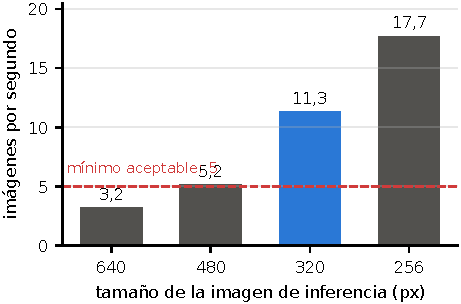
\includegraphics[width=0.52\textwidth]{fig_fps.pdf}
  \caption{Velocidad de procesamiento en la Raspberry Pi 5 seg\'un el tama\~no
  de la imagen de inferencia, incluyendo la captura.}
  \label{fig:fps}
\end{figure}

Con el lazo completo y el enlace serie real se midieron 11,2 ciclos por
segundo en banco. En el piso, registrando adem\'as la integridad de la imagen,
la velocidad fue de 10,5 a 10,7 ciclos por segundo, y de 9,6 a 10,0 al grabar
video; en las corridas de operaci\'on independiente estuvo entre 9,1 y 10,4.
El percentil 95 del per\'iodo del lazo estuvo entre 97 y 136 ms.

Con una sola fuente para todo el robot, la tensi\'on de 5 V ca\'ia durante la
inferencia: el lazo bajaba a 8,8 ciclos por segundo y la Raspberry Pi
recortaba su frecuencia el 43~\% del tiempo. Con dos fuentes separadas la
velocidad fue de 11,1 ciclos por segundo, sin ning\'un evento de baja
tensi\'on en 168 muestras, y la tensi\'on se mantuvo entre 4,91 y 5,13 V. En
150 s de inferencia continua la temperatura se estabiliz\'o entre 73 y
75~\grad C sin reducci\'on de frecuencia.

\subsubsection{Aproximaci\'on al objetivo}

La Figura~\ref{fig:tiras} (arriba) muestra la secuencia vista por la c\'amara
del robot, y la Figura~\ref{fig:aproximacion}, las variables registradas
durante una aproximaci\'on. El objetivo aparece en el borde derecho de la
imagen ($e_x=+0{,}63$); el robot avanza a la consigna m\'axima mientras gira,
el error lateral cruza la zona muerta en 1,3 s, el avance decrece a medida que
crece el \'area y el robot decide detenerse cuando $a$ alcanza 0,35, a los
2,1 s. En ese instante el ultras\'onico marca 28 cm; por inercia y por la
latencia, el robot queda detenido a 22 cm.

\begin{figure}[htbp]
  \centering
  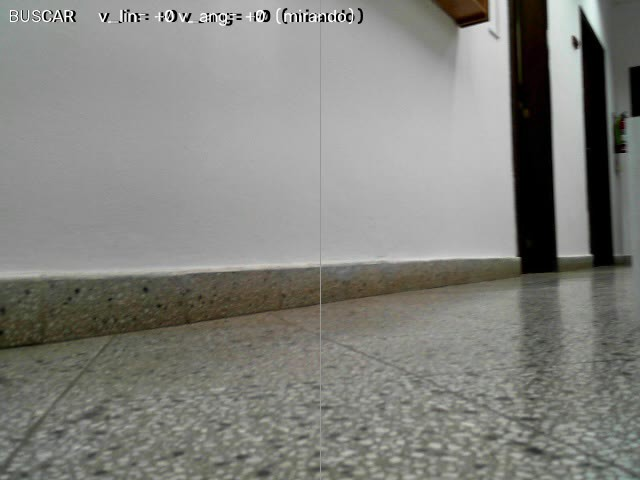
\includegraphics[width=0.19\textwidth]{oso_1.jpg}\hfill
  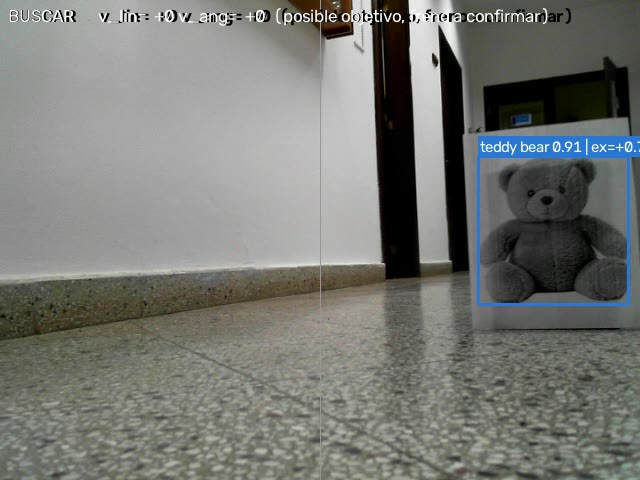
\includegraphics[width=0.19\textwidth]{oso_2.jpg}\hfill
  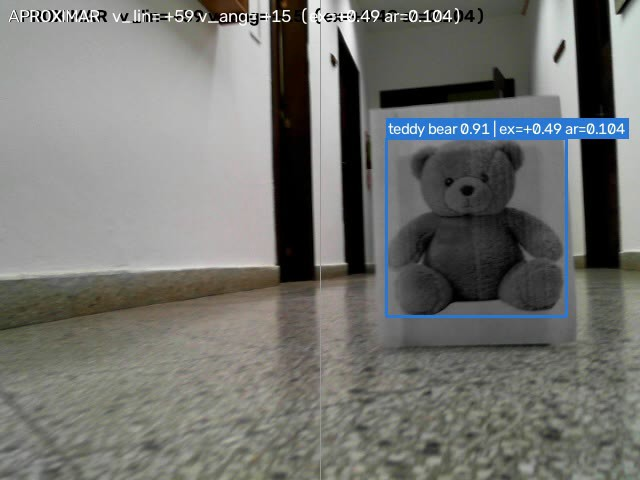
\includegraphics[width=0.19\textwidth]{oso_3.jpg}\hfill
  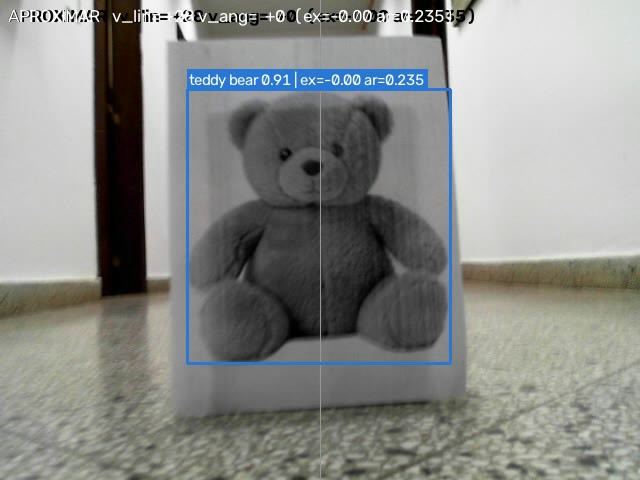
\includegraphics[width=0.19\textwidth]{oso_4.jpg}\hfill
  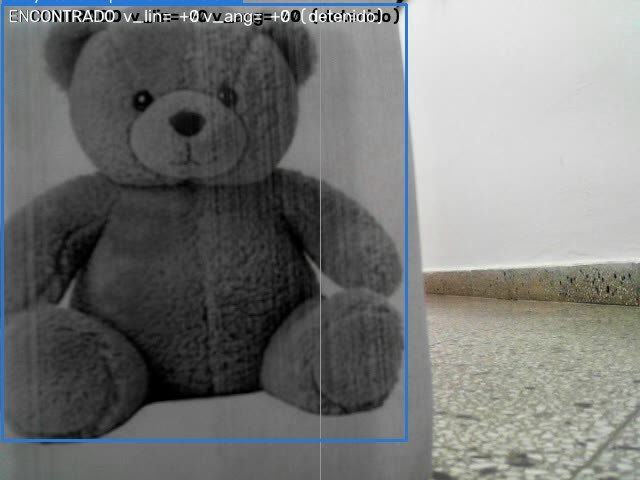
\includegraphics[width=0.19\textwidth]{oso_5.jpg}\\[3pt]
  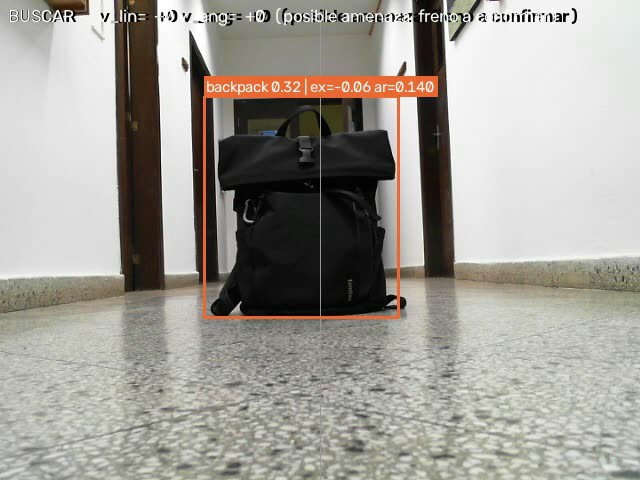
\includegraphics[width=0.19\textwidth]{huir_1.jpg}\hspace{0.0125\textwidth}%
  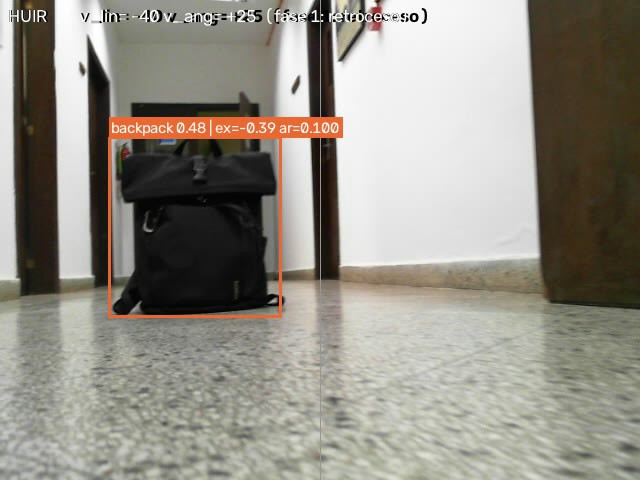
\includegraphics[width=0.19\textwidth]{huir_2.jpg}\hspace{0.0125\textwidth}%
  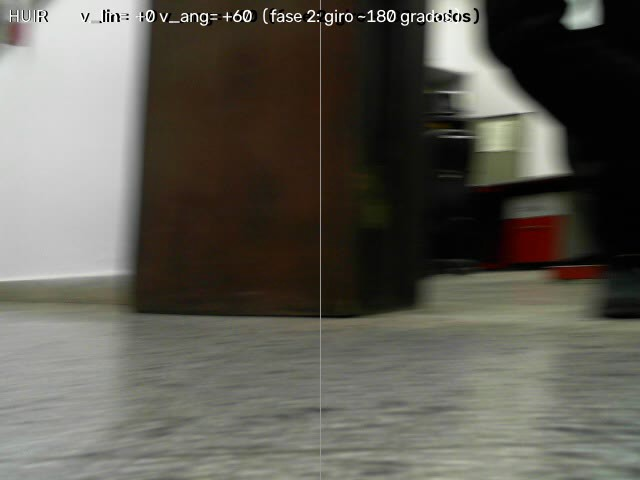
\includegraphics[width=0.19\textwidth]{huir_3.jpg}\hspace{0.0125\textwidth}%
  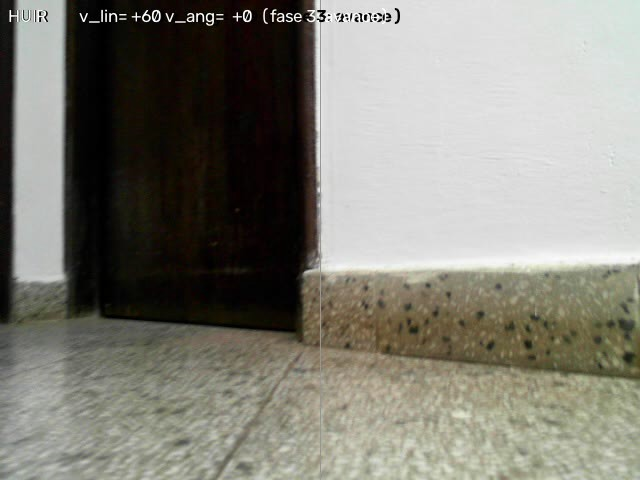
\includegraphics[width=0.19\textwidth]{huir_4.jpg}\hspace{0.2025\textwidth}
  \caption{Im\'agenes de la c\'amara del robot con las detecciones
  superpuestas. Arriba, aproximaci\'on: b\'usqueda, primera detecci\'on,
  avance, centrado y detenci\'on. Abajo, evasi\'on: detecci\'on de la
  amenaza, retroceso, giro y alejamiento.}
  \label{fig:tiras}
\end{figure}

\begin{figure}[htbp]
  \centering
  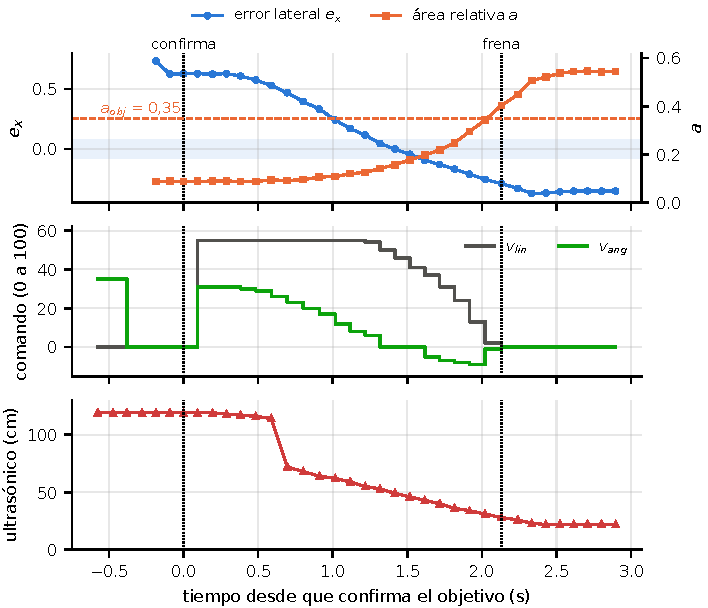
\includegraphics[width=0.74\textwidth]{fig_aproximacion.pdf}
  \caption{Una aproximaci\'on registrada (2 de octubre). Arriba: error
  lateral y \'area relativa del objetivo; la franja sombreada es la zona
  muerta del giro. Centro: consignas enviadas. Abajo: distancia del sensor
  ultras\'onico, que al principio apunta a otra superficie.}
  \label{fig:aproximacion}
\end{figure}

El objetivo se confirm\'o t\'ipicamente 0,2 s despu\'es de la primera imagen
en que apareci\'o (entre 0,11 y 0,40 s en las corridas registradas). El tiempo de aproximaci\'on, desde la confirmaci\'on hasta
la detenci\'on, fue de 1,7 a 3,1 s partiendo de alrededor de 1 m. El tiempo
total hasta encontrar depende de la orientaci\'on inicial: 3,1 s con el
objetivo de frente, y 15,0 y 17,0 s con el objetivo a 1 m y a 90\grad, porque
el barrido a pasos tarda unos 17 s por vuelta. El objetivo impreso se
detect\'o hasta 1,3 m, aproximadamente; ubicado a 2 m, el robot lo
encontr\'o reci\'en a los 65 s, cuando los avances de la b\'usqueda lo
acercaron.

\subsubsection{Evasi\'on y sensor ultras\'onico}

El robot decidi\'o huir t\'ipicamente 0,2 s despu\'es de la primera imagen que
conten\'ia la amenaza (entre 0,18 y 0,27 s cuando las tres im\'agenes que la
confirman son consecutivas). La maniobra completa dura 5,2 s. En la demostraci\'on con ambos objetos, la amenaza
colocada junto al objetivo durante una aproximaci\'on interrumpi\'o esta
\'ultima, como exige la prioridad.

La Tabla~\ref{tab:sonar} resume las mediciones del sensor ultras\'onico y la
Figura~\ref{fig:huida} muestra dos evasiones hacia una pared. Con un \'unico
umbral de 20 cm el robot interrumpi\'o el avance al leer 18 cm, pero como en
ese momento no frena sino que gira en el lugar, la lectura m\'inima baj\'o
hasta 11 cm. Con un umbral de esquive propio de 30 cm, el avance se
interrumpi\'o a 29 cm y la lectura no baj\'o de 27 cm. En el panel (b) se
observa adem\'as una limitaci\'on: al terminar el giro de la segunda fase, que
se hace sin informaci\'on de distancia, el robot ya estaba a 7 cm de un
obst\'aculo.

Las corridas de operaci\'on independiente, hechas en un espacio m\'as
reducido, mostraron los l\'imites del sensor. De nueve interrupciones del
avance, cinco ocurrieron al leer 29 o 30 cm y cuatro reci\'en al leer entre 16
y 20 cm, porque el obst\'aculo apareci\'o de un ciclo al siguiente, como ocurre
con una superficie abordada de forma oblicua. Y durante el giro de esquive la
lectura m\'inima lleg\'o a 3 cm en dos corridas, lo que indica que el robot
qued\'o pr\'acticamente en contacto con el obst\'aculo.

\begin{table}[htbp]
  \caption{Mediciones con el sensor ultras\'onico.}
  \label{tab:sonar}
  \centering
  \begin{tabular}{@{}L{6.4cm}L{6.0cm}@{}}
    \toprule
    \textbf{Prueba} & \textbf{Resultado} \\
    \midrule
    Robot quieto, caja a 30 cm & 30 cm, 120 lecturas v\'alidas de 120 \\
    Robot quieto en el piso, pared a 1,5 m & 153 cm, estable; sin ecos del piso \\
    Avance a consigna 40 hasta leer $\le$ 20 cm & orden de frenar a 19 cm; detenido a 16 cm \\
    Evasi\'on a consigna 60, umbral \'unico de 20 cm & interrumpe a 17--18 cm; m\'inimo 11--16 cm \\
    Evasi\'on a consigna 60, umbral de esquive 30 cm & interrumpe a 29 cm; m\'inimo 27 cm \\
    \'Idem, en operaci\'on independiente (9 casos) & interrumpe a 29--30 cm (5) o a 16--20 cm (4); m\'inimo 3 cm al girar \\
    Aproximaci\'on al objetivo & sin desv\'ios falsos; detenido a 22 cm \\
    \bottomrule
  \end{tabular}
\end{table}

\begin{figure}[htbp]
  \centering
  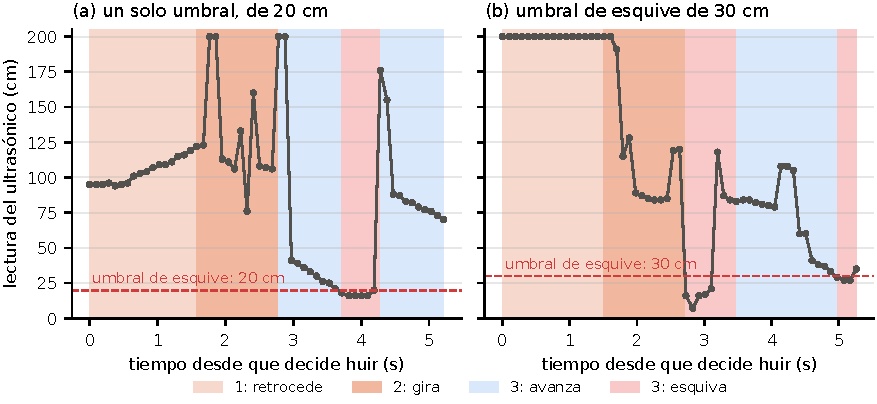
\includegraphics[width=0.98\textwidth]{fig_huida.pdf}
  \caption{Lectura del sensor ultras\'onico durante dos evasiones hacia una
  pared. El fondo indica la fase de la maniobra. Las lecturas mayores de 2 m,
  que corresponden a ``sin obst\'aculo'', se muestran recortadas en 200 cm.}
  \label{fig:huida}
\end{figure}

\subsubsection{Resumen de m\'etricas y de corridas}

La Tabla~\ref{tab:resultados} compara las m\'etricas con los objetivos
fijados antes de las pruebas, y la Tabla~\ref{tab:corridas} del
Ap\'endice~\ref{ap:material} detalla las 24 corridas en el piso.

\begin{table}[htbp]
  \caption{M\'etricas medidas frente a los objetivos definidos en el plan.}
  \label{tab:resultados}
  \centering
  \begin{tabular}{@{}L{4.0cm}L{2.4cm}L{5.8cm}@{}}
    \toprule
    \textbf{M\'etrica} & \textbf{Objetivo} & \textbf{Medido} \\
    \midrule
    Velocidad del lazo completo & $\ge$ 5 por segundo & 9,1 a 10,7 seg\'un la corrida \\
    Latencia de decisi\'on & registrar & $\sim$150 ms \\
    Alcance de detecci\'on del objetivo & hasta 2 m & $\sim$1,3 m (no cumple) \\
    Tiempo de confirmaci\'on & registrar & $\sim$0,2 s (0,11 a 0,40 s) \\
    Latencia de reacci\'on ante la amenaza & registrar & $\sim$0,2 s (0,18 a 0,27 s) \\
    Tiempo hasta encontrar & registrar & 3,1 s de frente; 15 a 17 s a 90\grad; 65 s a 2 m \\
    Distancia de parada & $\sim$30 cm & $\sim$30 cm con cinta; 22 cm seg\'un el ultras\'onico \\
    \'Exito de aproximaci\'on & $\ge$ 8 de 10 & 8 de 10 de puesta a punto; en operaci\'on independiente, 0 de 3 antes y 3 de 5 despu\'es del cambio en la b\'usqueda \\
    \'Exito de evasi\'on & $\ge$ 8 de 10 & 39 maniobras iniciadas; 2 corridas iniciales sin disparo (corregido); sin serie \\
    Prioridad de la evasi\'on & 10 de 10 & verificada sin hardware; 1 caso en el piso \\
    Parada ante p\'erdida de \'ordenes & $<$ 1 s & 0,5 s, verificada en hardware \\
    Im\'agenes da\~nadas $F$ & 0 & episodios el 1 de octubre; el 2 de octubre, 0 de 3675 a la ma\~nana y 33 de 3793 a la tarde \\
    \bottomrule
  \end{tabular}
\end{table}

De las 10 corridas de puesta a punto cuyo escenario inclu\'ia el objetivo, 8
terminaron en ENCONTRADO. Las dos restantes no son fallas de la conducta: en
una la c\'amara entregaba im\'agenes da\~nadas y la red no detect\'o nada, y
la otra se interrumpi\'o a los 52 s al advertirse que el sensor ultras\'onico
estaba desconectado. Las colisiones no se instrumentaron: con el umbral de
esquive de 30 cm, el registro no muestra lecturas inferiores a 27 cm
\emph{durante el avance} en ninguna corrida; antes de incorporar el sensor,
el operador observ\'o una evasi\'on que termin\'o contra una pared.

En las corridas de operaci\'on independiente el resultado fue distinto
(Tabla~\ref{tab:independiente}). En las tres primeras, con la amenaza a la
vista y poco espacio libre, el robot no lleg\'o al objetivo, y en la \'ultima
de ellas encaden\'o seis evasiones en 60 s: cuatro comenzaron unos 2 s
despu\'es de terminar la anterior, que es la duraci\'on del per\'iodo en que
la amenaza se ignora. Tras modificar el sentido de la b\'usqueda posterior a
la evasi\'on, el robot lleg\'o al objetivo en tres de cinco corridas y s\'olo
una de quince evasiones comenz\'o apenas terminada la anterior. En las otras
dos corridas sigui\'o huyendo cuatro y cinco veces en un minuto, ahora con
intervalos de 3 a 16 s: completaba parte del barrido, volv\'ia a encontrar la
amenaza y no lleg\'o a detectar el objetivo. Las condiciones de estas
corridas no se controlaron, por lo que la comparaci\'on es indicativa.

\begin{table}[htbp]
  \caption{Corridas de operaci\'on independiente, antes y despu\'es de
  modificar el sentido de la b\'usqueda posterior a la evasi\'on.}
  \label{tab:independiente}
  \centering
  \begin{tabular}{@{}L{6.2cm}L{2.8cm}L{2.8cm}@{}}
    \toprule
     & \textbf{Antes} & \textbf{Despu\'es} \\
    \midrule
    Corridas & 3 & 5 \\
    Llegaron al objetivo & 0 & 3 \\
    Evasiones iniciadas & 8 & 15 \\
    Evasiones iniciadas menos de 2,5 s despu\'es de terminar la anterior & 4 & 1 \\
    \bottomrule
  \end{tabular}
\end{table}

\subsubsection{Integridad de la imagen}

El 1 de octubre, con el robot quieto, 69 de 71 im\'agenes llegaron con
franjas grises, y la red no detect\'o el objetivo ubicado a 1 m
(Figura~\ref{fig:imagen}). El episodio se repiti\'o de forma intermitente con
los motores detenidos e incluso sin alimentaci\'on de motores, y ces\'o sin
intervenci\'on: en las ocho corridas siguientes no hubo ninguna imagen
da\~nada en 2104. El registro del sistema operativo mostr\'o que se trataba de
paquetes USB perdidos. El 2 de octubre, tras reinsertar el conector de la
c\'amara ---que se hab\'ia soltado--- y con las bater\'ias reci\'en cargadas,
no hubo im\'agenes da\~nadas en las 3675 de la ma\~nana. Como ambas
condiciones cambiaron a la vez, la causa no qued\'o aislada. Esa misma tarde
las franjas reaparecieron en dos de las ocho corridas de operaci\'on
independiente (24 de 569 im\'agenes en una y 9 de 600 en otra), lo que
confirma que el problema sigue presente.

\begin{figure}[htbp]
  \centering
  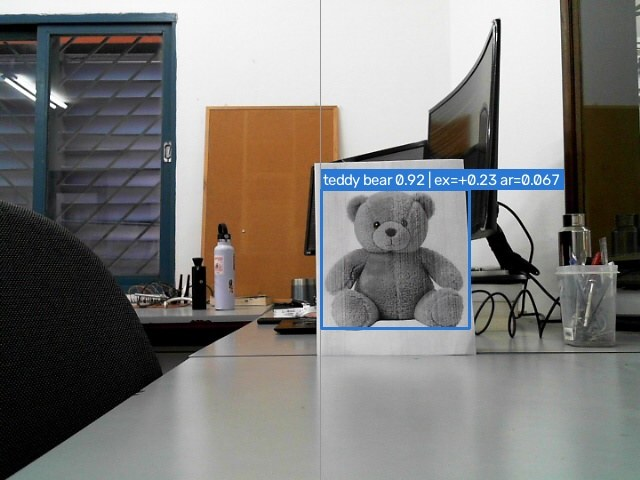
\includegraphics[width=0.30\textwidth]{img_sana.jpg}\hspace{4mm}%
  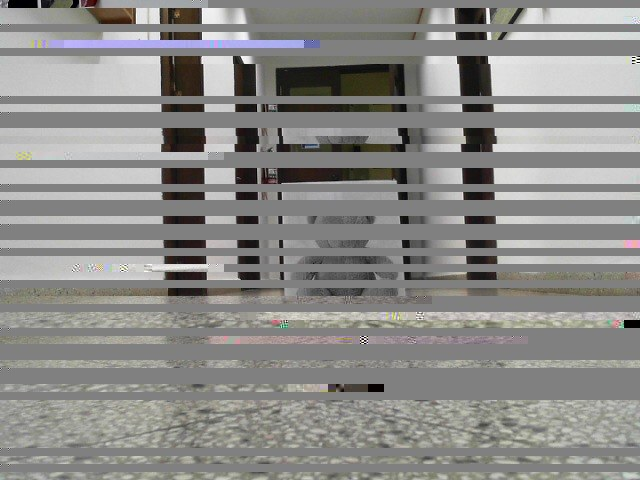
\includegraphics[width=0.30\textwidth]{img_rota_37.jpg}\hspace{4mm}%
  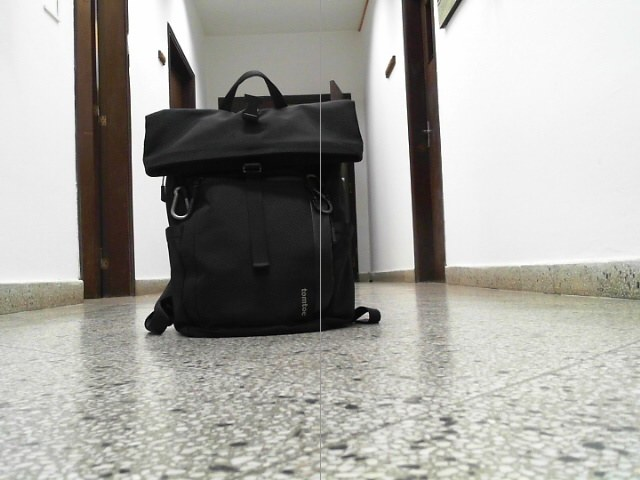
\includegraphics[width=0.30\textwidth]{mochila.jpg}
  \caption{Izquierda: imagen \'integra, con el objetivo detectado. Centro:
  imagen da\~nada por p\'erdida de paquetes USB, con el robot quieto; el
  objetivo est\'a detr\'as de las franjas. Derecha: la mochila vista desde el
  robot, que el modelo clasifica como \cod{suitcase}.}
  \label{fig:imagen}
\end{figure}

\subsection{Discusi\'on y limitaciones}\label{subsec:discusion}

\textbf{Cumplimiento de los objetivos.} El robot realiza las conductas
previstas con todo el c\'omputo a bordo y con m\'as del doble de la velocidad
de procesamiento m\'inima. La arquitectura de dos niveles cumpli\'o su
funci\'on: ning\'un cambio en la calibraci\'on de los motores oblig\'o a
modificar la ley de control, y la parada segura actu\'o cada vez que el
programa de alto nivel se detuvo.

\textbf{El contexto de validez de las mediciones.} El hallazgo m\'as
repetido del trabajo es que un valor medido deja de ser v\'alido fuera de las
condiciones en que se obtuvo. La calibraci\'on de la tracci\'on, exacta al
1~\% con las ruedas en el aire, no mov\'ia una de las ruedas con el robot
apoyado, porque le asignaba el menor ciclo de trabajo justamente a la rueda
de menor par; hubo que recalibrar en el piso
(Tabla~\ref{tab:calibracion}). La velocidad de giro de 165\grad/s, medida en
r\'egimen sobre varias vueltas, produjo unos 110\grad{} en la fase de giro de
la evasi\'on, que dura alrededor de un segundo y parte de la marcha atr\'as.
La etiqueta \cod{backpack} es correcta para las im\'agenes con que se
entren\'o la red, pero la misma mochila vista desde 10 cm del piso es, para
el modelo, una valija. Y la relaci\'on entre el giro de b\'usqueda y la
detecci\'on, supuesta al dise\~nar, s\'olo se resolvi\'o midiendo con la
propia c\'amara cu\'anto se desplaza la escena en cada paso. La respuesta
metodol\'ogica fue registrar junto a cada par\'ametro las condiciones en que
se midi\'o y probar una capa por vez.

\textbf{Valor de la verificaci\'on sin hardware.} El banco de verificaciones
detect\'o defectos antes de que tuvieran consecuencias f\'isicas, como el
encadenamiento de evasiones por la persistencia de la confirmaci\'on
temporal. Tambi\'en mostr\'o su l\'imite: una comprobaci\'on exig\'ia que una
detecci\'on no confirmada de la amenaza no detuviera el barrido, se cumpl\'ia
siempre y era la causa de que el robot no huyera en el piso. Una
verificaci\'on asegura que el c\'odigo hace lo decidido, no que la decisi\'on
fuera correcta.

\textbf{Limitaciones.}
\begin{itemize}
  \item \emph{Evaluaci\'on.} No se complet\'o la serie de 10 repeticiones por
        escenario; las tasas de la Tabla~\ref{tab:resultados} provienen de
        pocas corridas con par\'ametros que cambiaron entre ellas.
  \item \emph{Ciclo de evasiones.} Con la amenaza siempre a la vista y una
        pared cercana, el robot qued\'o en un ciclo: al huir encontraba la
        pared, giraba para esquivarla hasta quedar nuevamente orientado
        hacia la amenaza ---en tres casos incluso avanz\'o hacia ella--- y
        volv\'ia a huir al terminar el per\'iodo de 2 s. Se modific\'o el
        sentido del barrido posterior a la evasi\'on: ahora es aleatorio, o
        contrario al lado de la amenaza si esta queda a la vista. En las
        cinco corridas posteriores el ciclo de 2 s pr\'acticamente
        desapareci\'o y el robot lleg\'o al objetivo en tres, pero en las
        otras dos sigui\'o huyendo de forma repetida sin encontrarlo. El giro
        de esquive, que es la causa de fondo, no se modific\'o, y la
        comparaci\'on no proviene de una serie controlada.
  \item \emph{Sensado de obst\'aculos.} El sensor s\'olo cubre el frente. El
        retroceso y el giro de la evasi\'on se hacen sin informaci\'on de
        distancia, y una pared abordada de forma muy oblicua no se detecta
        hasta estar a unos 20 cm, porque el eco se refleja en otra
        direcci\'on: en espacios reducidos el robot lleg\'o a quedar a 3 cm
        de un obst\'aculo mientras giraba. Los tres par\'ametros asociados al
        sensor se ajustaron con una corrida cada uno.
  \item \emph{Alcance y dependencia del objeto.} El objetivo se detecta
        hasta 1,3 m con la imagen de 320 p\'ixeles. La distancia de parada
        depende del tama\~no del objeto con que se calibr\'o.
  \item \emph{Falsos positivos de la amenaza.} El umbral reducido a 0,20
        produce detecciones aisladas sobre objetos oscuros grandes. La
        confirmaci\'on temporal impidi\'o que desencadenaran una evasi\'on en
        las pruebas, pero el resultado depende del entorno.
  \item \emph{Tracci\'on a lazo abierto.} Sin codificadores, el robot se
        desv\'ia al acelerar y al frenar, y queda con el objetivo descentrado
        algunos grados al detenerse.
  \item \emph{Integridad de la imagen.} La causa de la p\'erdida de paquetes
        USB no qued\'o aislada y el problema reapareci\'o la \'ultima tarde;
        el sistema lo detecta y lo registra, pero no lo corrige.
  \item \emph{Dependencia del enlace de operaci\'on.} Si se corta la sesi\'on
        remota desde la que se lanza una corrida, el programa puede seguir
        ejecut\'andose hasta su l\'imite de tiempo; la parada autom\'atica
        protege ante la ca\'ida del programa, no ante la del enlace.
\end{itemize}

\section{Conclusiones}\label{sec:conclusiones}

Se construy\'o un robot m\'ovil que busca un objeto, se aproxima a \'el y se
detiene a unos 30 cm, y que evade otro objeto con prioridad sobre la
aproximaci\'on, con la detecci\'on ejecutada a bordo en una Raspberry Pi 5 a
unas 10 im\'agenes por segundo. El objetivo general se cumpli\'o en cuanto
a la integraci\'on de percepci\'on, decisi\'on y actuaci\'on en el robot
f\'isico; la evaluaci\'on cuantitativa del \'exito de cada conducta qued\'o
incompleta, porque no se realizaron las series de repeticiones previstas.

Los resultados m\'as relevantes son la latencia de decisi\'on de unos 150 ms,
la confirmaci\'on de un objeto y la reacci\'on ante la amenaza en 0,2 s, la
aproximaci\'on desde 1 m en 2 a 3 s y la interrupci\'on del avance a 29 cm de
un obst\'aculo frontal. La separaci\'on en dos niveles, la verificaci\'on del
comportamiento sin hardware y el registro ciclo por ciclo fueron las
decisiones que m\'as contribuyeron a llegar a ese resultado y a poder
explicarlo.

Como trabajo futuro se propone: completar las series de 10 corridas por
escenario, incluida una que eval\'ue de forma controlada el cambio en el
sentido de b\'usqueda; acotar el giro de esquive durante la evasi\'on; aislar
la causa de la p\'erdida de im\'agenes; a\~nadir sensado de distancia lateral
y trasero; incorporar codificadores para cerrar un lazo de velocidad
por rueda; aumentar el alcance de detecci\'on usando una imagen mayor s\'olo
mientras el robot est\'a detenido en la b\'usqueda; y evaluar un modelo
ajustado con im\'agenes tomadas desde la altura de la c\'amara del robot.

\section*{Contribuci\'on de los integrantes}

Los dos integrantes participaron en la definici\'on del problema y del
alcance, en el montaje y el cableado del robot, en las decisiones de dise\~no,
en las pruebas f\'isicas y las observaciones en el piso, y en la revisi\'on del
software, los resultados y la documentaci\'on.

\section*{Disponibilidad del c\'odigo y los datos}

El c\'odigo fuente, el firmware, los registros de las corridas, los videos y
la documentaci\'on est\'an disponibles en un repositorio p\'ublico, bajo la
licencia AGPL-3.0:
\url{https://github.com/fedemoranf-alt/AguaraBot-RoboticaIA-MscIA}. El
repositorio contiene:
\cod{src/} (software de la Raspberry Pi, incluido el banco de
verificaciones), \cod{firmware/} (firmware del ESP32, con su historial de
versiones), \cod{scripts\_pi/} (puesta en marcha y operaci\'on), \cod{logs/}
(un archivo CSV y uno JSON por corrida), \cod{media/} (videos tomados por la
c\'amara del robot) y los documentos \cod{HARDWARE.md} (an\'alisis
el\'ectrico y mediciones) y \cod{GUIA\_PRESENTACION.md} (gu\'ia de
operaci\'on). Las
verificaciones sin hardware se reproducen con \cod{python
prueba\_estados.py} desde \cod{src/}; las figuras de este informe, con
\cod{python generar\_figuras.py}; y una corrida en el robot, con
\cod{demo.sh correr}, seg\'un la gu\'ia de operaci\'on.

\section*{Uso de herramientas de inteligencia artificial generativa}

Durante todo el proyecto se utiliz\'o un asistente basado en un modelo de
lenguaje (Claude, de Anthropic, mediante la herramienta Claude Code). Se lo
emple\'o para la asistencia en la programaci\'on del firmware y del software
de alto nivel.
% -----------------------------------------------------------------------------
\begin{thebibliography}{12}

\bibitem{ref:yolo}
Redmon, J., Divvala, S., Girshick, R., Farhadi, A.: You only look once:
unified, real-time object detection. In: Proceedings of the IEEE Conference on
Computer Vision and Pattern Recognition (CVPR), pp. 779--788 (2016).
\url{https://doi.org/10.1109/CVPR.2016.91}

\bibitem{ref:yolorev}
Terven, J., C\'ordova-Esparza, D.-M., Romero-Gonz\'alez, J.-A.: A comprehensive
review of YOLO architectures in computer vision: from YOLOv1 to YOLOv8 and
YOLO-NAS. Machine Learning and Knowledge Extraction \textbf{5}(4), 1680--1716
(2023). \url{https://doi.org/10.3390/make5040083}

\bibitem{ref:yolov8}
Jocher, G., Chaurasia, A., Qiu, J.: Ultralytics YOLO (2023).
\url{https://github.com/ultralytics/ultralytics}

\bibitem{ref:coco}
Lin, T.-Y., Maire, M., Belongie, S., Hays, J., Perona, P., Ramanan, D.,
Doll\'ar, P., Zitnick, C.L.: Microsoft COCO: common objects in context. In:
Computer Vision -- ECCV 2014. Lecture Notes in Computer Science, vol. 8693,
pp. 740--755. Springer, Cham (2014).
\url{https://doi.org/10.1007/978-3-319-10602-1_48}

\bibitem{ref:braitenberg}
Braitenberg, V.: Vehicles: Experiments in Synthetic Psychology. MIT Press,
Cambridge (1984)

\bibitem{ref:brooks}
Brooks, R.A.: A robust layered control system for a mobile robot. IEEE Journal
on Robotics and Automation \textbf{2}(1), 14--23 (1986).
\url{https://doi.org/10.1109/JRA.1986.1087032}

\bibitem{ref:arkin}
Arkin, R.C.: Behavior-Based Robotics. MIT Press, Cambridge (1998)

\bibitem{ref:visualservo}
Chaumette, F., Hutchinson, S.: Visual servo control. I. Basic approaches. IEEE
Robotics \& Automation Magazine \textbf{13}(4), 82--90 (2006).
\url{https://doi.org/10.1109/MRA.2006.250573}

\bibitem{ref:siegwart}
Siegwart, R., Nourbakhsh, I.R., Scaramuzza, D.: Introduction to Autonomous
Mobile Robots, 2nd edn. MIT Press, Cambridge (2011)

\bibitem{ref:l298}
STMicroelectronics: L298 -- Dual full-bridge driver. Hoja de datos

\bibitem{ref:ping}
Parallax Inc.: PING))) Ultrasonic Distance Sensor (\#28015). Gu\'ia del
producto

\bibitem{ref:esp32}
Espressif Systems: ESP32 Series Datasheet

\end{thebibliography}

\begin{appendices}

\section{Material complementario}\label{ap:material}

\subsection{Calibraci\'on de la tracci\'on}

La Tabla~\ref{tab:calibracion} compara la calibraci\'on obtenida con las
ruedas en el aire con la que qued\'o cargada tras recalibrar con el robot
apoyado. Los valores son cuentas del ciclo de trabajo, sobre un m\'aximo de
1023.

\begin{table}[!htbp]
  \caption{Calibraci\'on de la tracci\'on, rueda izquierda / rueda derecha.}
  \label{tab:calibracion}
  \centering
  \begin{tabular}{@{}L{5.2cm}L{3.2cm}L{3.2cm}@{}}
    \toprule
    \textbf{Par\'ametro} & \textbf{En el aire} & \textbf{En el piso} \\
    \midrule
    Piso de la recta $d_{\min}$ & 125 / 112 & 300 / 230 \\
    Techo de la recta $d_{\max}$ & 238 / 352 & 413 / 470 \\
    Pulso de arranque & 290 / 220 & 380 / 280 \\
    Duraci\'on del pulso de arranque & 80 ms & 150 ms \\
    \bottomrule
  \end{tabular}
\end{table}

Con la calibraci\'on en el aire, el rango \'util de velocidad de cada rueda
es de 0,091 a 0,380 m/s. La carga del robot desplaza ambas rectas hacia
arriba sin cambiar su pendiente. Con la calibraci\'on de piso, un avance
cronometrado recorri\'o 57 cm frente a los 57 cm previstos. El giro en el
lugar alcanza en r\'egimen 124\grad/s con una consigna de 35 y 165\grad/s con
una consigna de 60.

\clearpage
\subsection{Corridas en el piso}

La Tabla~\ref{tab:corridas} lista las 24 corridas de comportamiento
registradas en el piso, en orden cronol\'ogico. Las diez primeras
corresponden al 1 de octubre, antes de incorporar el sensor ultras\'onico;
las seis siguientes, a la ma\~nana del 2 de octubre, ya con el sensor y el
zumbador; y las ocho \'ultimas son las de operaci\'on independiente, de esa
tarde: tres anteriores y cinco posteriores al cambio en el sentido de la
b\'usqueda.

\begin{table}[!htbp]
  \caption{Corridas en el piso. ``Enc.'' es el instante en que se alcanz\'o el
  estado ENCONTRADO; ``c/s'' son ciclos del lazo por segundo.}
  \label{tab:corridas}
  \centering
  \footnotesize
  \begin{tabular}{@{}L{1.4cm}L{3.3cm}L{0.5cm}L{0.6cm}L{0.75cm}L{4.3cm}@{}}
    \toprule
    \textbf{D\'ia, hora} & \textbf{Escenario} & \textbf{s} & \textbf{c/s} & \textbf{Enc.} & \textbf{Resultado} \\
    \midrule
    1/10 15:21 & Objetivo a 1 m, 90\grad & 25 & 9,7 & --- & Sin detecciones: imagen da\~nada \\
    1/10 16:02 & Objetivo de frente, $\sim$1 m & 15 & 10,0 & 3,1 s & Llega; 37 cm con cinta ($a_{obj}$ anterior) \\
    1/10 16:23 & Objetivo a 1 m, 90\grad & 30 & 9,8 & 17,0 s & Llega; termina descentrado \\
    1/10 16:29 & Objetivo a 1 m, 90\grad & 30 & 9,9 & 15,0 s & Llega, centrado \\
    1/10 16:40 & Amenaza a 1 m & 12 & 10,0 & --- & No huye: el barrido no se deten\'ia \\
    1/10 16:43 & Amenaza a 1 m & 12 & 10,0 & --- & No huye: confianza bajo el umbral \\
    1/10 16:50 & Amenaza a 1 m & 12 & 9,8 & --- & Huye; gira $\sim$110\grad \\
    1/10 16:54 & Amenaza a 1 m & 12 & 9,6 & --- & Evasi\'on completa \\
    1/10 17:07 & Objetivo a $\sim$2 m & 90 & 9,9 & 65,3 s & Llega; lo pierde una vez \\
    1/10 17:17 & Objetivo y amenaza & 90 & 9,9 & 85,4 s & 4 evasiones; llega al final \\
    \midrule
    2/10 10:34 & Amenaza; pared a 1 m & 30 & 10,6 & 29,3 s & 1 evasi\'on; el avance termina a 27 cm \\
    2/10 10:36 & Amenaza; pared a 0,8 m & 30 & 10,7 & --- & 3 evasiones; esquiva a 18 cm \\
    2/10 10:41 & Objetivo a 1,5--2 m & 60 & 10,5 & 58,8 s & 2 evasiones; llega \\
    2/10 10:54 & Objetivo y amenaza & 52 & 10,7 & --- & Sensor desconectado; interrumpida \\
    2/10 10:59 & Objetivo y amenaza & 90 & 10,7 & 21,0 s & 2 evasiones; esquiva a 29 cm; llega \\
    2/10 11:07 & Objetivo y amenaza & 90 & 9,9 & 8,0 s & 1 evasi\'on; llega (con video) \\
    \midrule
    2/10 13:46 & Independiente, antes & 34 & 10,2 & --- & Permanece en b\'usqueda \\
    2/10 13:48 & Independiente, antes & 60 & 9,1 & --- & 2 evasiones; no llega \\
    2/10 13:50 & Independiente, antes & 60 & 9,1 & --- & 6 evasiones en ciclo \\
    \midrule
    2/10 14:03 & Independiente, despu\'es & 14 & 10,3 & 6,9 s & 1 evasi\'on; llega \\
    2/10 14:04 & Independiente, despu\'es & 60 & 10,4 & --- & 4 evasiones; no llega \\
    2/10 14:19 & Independiente, despu\'es & 60 & 9,5 & --- & 5 evasiones; no llega; im\'agenes da\~nadas \\
    2/10 14:20 & Independiente, despu\'es & 45 & 9,1 & 5,2 s & Llega; 1 evasi\'on; vuelve a llegar \\
    2/10 14:21 & Independiente, despu\'es & 60 & 10,0 & 55,1 s & 4 evasiones; llega \\
    \bottomrule
  \end{tabular}
\end{table}

\subsection{Asignaci\'on de pines del ESP32}

La Tabla~\ref{tab:pines} indica las conexiones del microcontrolador. Los pines
del sensor ultras\'onico y del zumbador se eligieron entre los accesibles en
la placa de pruebas; los de s\'olo entrada quedan reservados para los
codificadores.

\begin{table}[!htbp]
  \caption{Conexiones del ESP32.}
  \label{tab:pines}
  \centering
  \begin{tabular}{@{}L{4.6cm}L{2.2cm}L{5.4cm}@{}}
    \toprule
    \textbf{Se\~nal} & \textbf{GPIO} & \textbf{Observaci\'on} \\
    \midrule
    L298N ENA / IN1 / IN2 & 25 / 26 / 27 & Canal A: rueda derecha \\
    L298N ENB / IN3 / IN4 & 13 / 33 / 32 & Canal B: rueda izquierda \\
    Ultras\'onico, l\'inea de se\~nal & 12 & Con divisor 1 k$\Omega$ / 2 k$\Omega$ \\
    Zumbador & 14 & Activo, conexi\'on directa \\
    Codificadores (reservados) & 34, 35, 36, 39 & Sin conectar; s\'olo entrada \\
    \bottomrule
  \end{tabular}
\end{table}

\end{appendices}

\end{document}
